\documentclass[10pt, fullpage, a4paper, titlepage]{article}
\usepackage{graphicx, latexsym}
\usepackage{setspace}
\usepackage{apalike}
\usepackage{amssymb, amsmath, amsthm}
\usepackage{bm}
\usepackage{epstopdf}
\usepackage[]{hyperref}
\usepackage{booktabs}
\usepackage{subfigure}
 \hypersetup{
    pdftitle={Markup languages - 1},
    pdfauthor={Ilaria Francesca Lunardelli},
    pdfsubject={cool stuff},
    pdfkeywords={koala, chuck norris},
    bookmarksnumbered=true,     
    bookmarksopen=true,         
    bookmarksopenlevel=1,       
    colorlinks=true,            
    pdfstartview=Fit,           
    pdfpagemode=UseOutlines,      
    pdfpagelayout=TwoPageRight
    }

%\singlespacing
    %\onehalfspacing
    \doublespacing

\title{Markup languages - 1\\ \First home exercise}
\author{Ilaria Francesca Lunardelli }
%\date{\today}
\date{}


\begin{document}

\maketitle

\newpage
 \section*{Abstract}
    text of abstract
    
\section{Introduction}
Cervical cancer is the fourth most common cancer among women globally, with an estimated 604000 new cases and 342000 deaths (World Health Organization, 2022). 

The research question we aim to answer is “What are the most relevant predictors of cervical cancer and is there evidence for saying that their effects are different from zero?”.


\subsection{Data-set}
  The data-set chosen for this assignment is called “Cervical cancer (Risk Factors)”, it was collected at the University Hospital in Caracas, Venezuela and it is available on Kaggle (UCI, 2017). The data-set includes 37 variables which measure demographic information, habits and medical records of 858 patients. Several missing data values were present in the original data-set and have been removed for simplicity reason, leaving us with 669 observations. 
The original data-set includes four different variables that indicate the result of different medical tests that are used to recognize the presence of cervical cancer (Hinselmann, Schiller, Cytology and Biopsy). I decided to aggregate these four variables to obtain one outcome variable that indicates whether the person has ever been diagnosed with the cancer in any of the tests (0 = no cancer diagnosis, 1 = cancer diagnosis). Moreover, among the several variables of the original data-set I discarded the variables that are redundant and those that are constant. The end result was a data-set with the following 7 variables that are well-known risk factors in literature on cervical cancer:
\begin{itemize}
    \item 	Age: A study conducted by Juneja et al. (2003), revealed that more than 75% of the detected cervical cancer cases are observed in women aged above 35.
\item 	Sexual partners: Brinton et al. (1993) discovered that women with 2 or more partners have a RR of 1,5% compared to women with only 1 partner or less.
\item 	Smoke: Multiple studies found a positive correlation between smoking and the development of cervical cancer (Roura et al. 2013) (Juneja et al. 2003). In particular, Lukac et al. (2018) found that women who smoke have a 2 to 4 times higher risk of having cervical cancer compared to women that don’t. 
\item 	Age of first sexual intercourse: Brinton et al. (1993) found in their study that women who experienced their first sexual intercourse before the age of 16 have twice the risk of developing cervical cancer compared to women who experienced it at the age of 20 or later.
\item 	Number of pregnancies: Thulaseedharan et al. (2012) indicate that the risk of having cervical cancer is 7.1 times higher for women who had more than 4 pregnancies compared to women who have never been pregnant.
\item 	Usage of hormonal contraceptives: Zhang et al (2020) found that the use this kind of contraceptives for a period of at least 5 years would double the risk of cancer.
\item 	HIV: STDs, especially HIV, are found to be high risk factors (Zhang et al 2020). Cervical cancer is 6.8 times more likely to develop in HIV positive women than in women who are not affected by HIV (Chambuso R.S. et al. 2016).
\end{itemize}
All of these variables were turned into dichotomous / categorical features in compliance with the aforementioned literature. The cited literature was also used to create informative priors.


\section{Analytic strategy}
For the first bullet I chose to build a logistic regression model in order to determine which variables predict the cancer, since the outcome variable is dichotomous. The choice of using a Gibbs sampler is to have a faster convergence than a MH algorithm and to not have to worry about acceptance of the proposed values for our coefficients.

The model we used comes from the paper “Bayesian Inference for Logistic Models Using Pólya-Gamma Latent Variables” by Polson et al. (2013). The Gibbs sampler makes use of the Pólya-Gamma (PG) distribution as a latent variable to sample from the posterior distribution of the beta coefficients of a logistic regression. 
Let $yi$ be the number of successes, $n_i$ the number of trials and 
$x_i = (x_{i1}, ..., x_{ip})$ the vector of covariates for observation $i \in {1, ..., N}$. Let  $yi \thicksim Binom (n_i,1 / {1 +e^{-\psi_i} }$, where $\psi_i=x_i^T \beta $ are the log odds of success. Let $\beta$ have a gaussian prior, $\beta \thicksim N (b, B)$.
\\ The sampler requires only two steps that are the following: 
\begin{itemize}
    \item Step 1. Data augmentation with Pólya-Gamma
    \begin{equation*}
\label{eq1}
(\omega_i|\beta) \sim PG(1,x_i^T\beta)
\end{equation*}
    \item Step 2. Sample from the posterior distribution of $\beta$
     \begin{equation*}
\label{eq2}
(\beta \mid y, \omega_i )  ~ N(m_\omega,V_\omega)
\end{equation*}
 
where
\begin{equation*}
\label{eq3}
V_\omega=(X^T \Omega X+B^{-1} )^{-1}
\end{equation*}
\begin{equation*}
\label{eq4}
m_\omega=V_\omega  (X^T k+B^(-1) b) 
\end{equation*}
\\
$k=y_1-1/2$ and $\Omega$ is the diagonal matrix of $\omega_l$’s. 
The samples drawn in step 2 are indeed extractions of the beta coefficients of our logistic regression. 

\end{itemize}
\newpage
\begin{figure}[h]
     \begin{center}
%
        \subfigure[Histogram]{%
            \label{fig:first}
            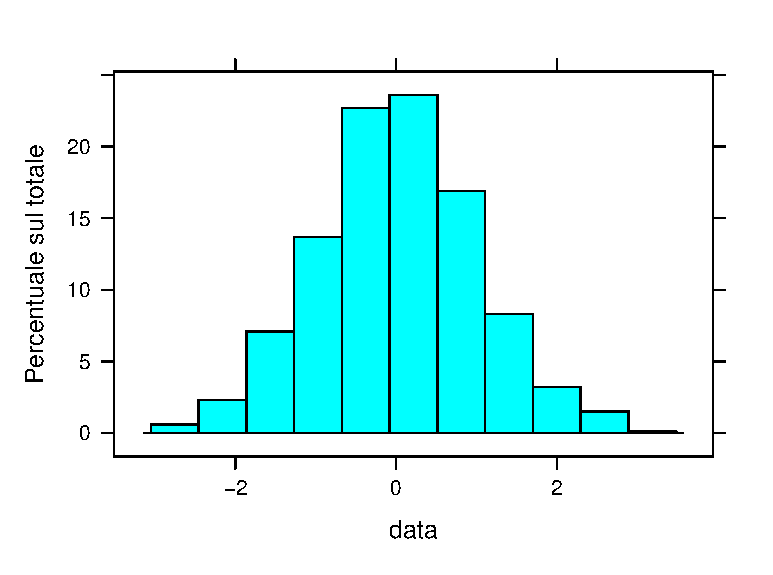
\includegraphics[width=0.35\textwidth]{Rplot1.pdf}
        }%
        \subfigure[Densityplot]{%
           \label{fig:second}
           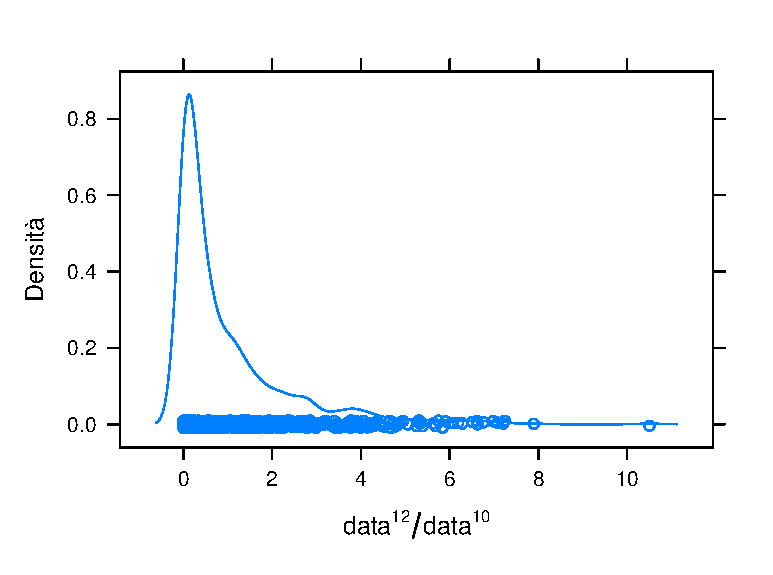
\includegraphics[width=0.35\textwidth]{Rplot2.pdf}
        }\\ %  ------- End of the first row ----------------------%
        \subfigure[Stripplot]{%
            \label{fig:third}
            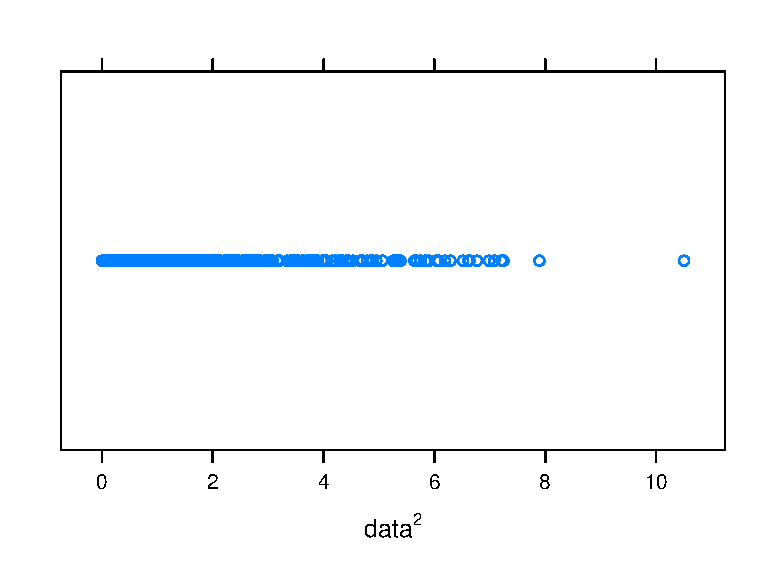
\includegraphics[width=0.35\textwidth]{Rplot3.pdf}
        }%
        \subfigure[Boxplot]{%
            \label{fig:fourth}
            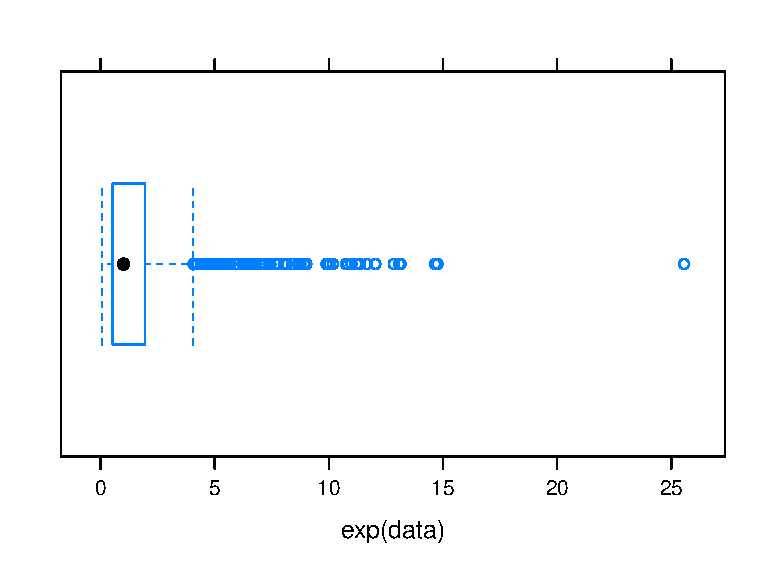
\includegraphics[width=0.35\textwidth]{Rplot4.pdf}
        }%
%
    \end{center}
    \caption{%
        Different plots of the same data, sometimes transformed. No particular objective other than it being an exercise.
     }%
   \label{fig:subfigures}
\end{figure}
 
 \begin{table}[h]
\centering
\caption{The same data, but now in a table. Only the first nine rows are displayed.}
\label{tab:my-table}
\begin{tabular}{@{}ccccc@{}}
\toprule
  & data  & squared 1 & squared 2 & exponent \\ \midrule
1 & -0.56 & 0.31      & 0.31      & 0.57     \\
2 & -0.23 & 0.05      & 0.05      & 0.79     \\
3 & 1.56  & 2.43      & 2.43      & 4.75     \\
4 & 0.07  & 0.00      & 0.00      & 1.07     \\ 
5 & 0.13  & 0.02      & 0.02      & 1.14     \\
6 & 1.72  & 2.94      & 2.94      & 5.56     \\
7 & 0.46  & 0.21      & 0.21      & 1.59     \\
8 & -1.27 & 1.60      & 1.60      & 0.28     \\
9 & -0.69 & 0.47      & 0.47      & 0.50    
\end{tabular}
\end{table}

\newpage
\section{AI generated fairytale}
The Enchanted Garden and the Magical Dove

Once, in a land covered by mists and whispers, there lay an enchanting garden hidden behind a great stone wall. No one knew who had built the wall or why, but one thing was for certain – nobody had ever seen what was behind it.

A little boy named Peter lived in a village nearby. Fuelled by curiosity and tales of magical creatures, he often dreamt of the wonders that the walled garden might hold. One day, unable to resist its lure any longer, he decided to find a way in.

As he approached the towering stone barrier, he noticed a tiny gap just big enough for him to peek through. The garden inside was bathed in a shimmering golden light, unlike any he had ever seen. To his amazement, in the center stood a magnificent tree with leaves that glittered as if they were made of starlight. And resting on one of its branches was a dove, glowing with the same luminous hue.

Before he could process this beautiful sight, the dove spoke to his in a voice as soft as the wind, "To enter the garden, one must share a pure and selfless desire."

Peter, with his heart pounding, whispered his wish, "I wish for everyone in my village to be happy and free from suffering."

The massive stone door, seemingly of its own accord, began to open. The luminous dove flew to Peter and rested on his shoulder. "Your wish is genuine, and so you may enter," it said.

Inside, the garden was more wondrous than Peter had ever imagined. Flowers sang in soft harmonies, and a gentle breeze carried the sweetest of fragrances. Every step he took made the grass shimmer with colors she'd never seen before.

The dove explained that this was an Enchanted Garden, a place where one’s purest wishes could come true. But, there was a catch. To make his wish a reality, Peter had to plant a seed from the magical tree in his village and care for it with unwavering love and dedication.

Peter accepted the challenge. With the seed safely tucked in his pocket and the dove guiding her, he returned to his village.

Years went by, and with Peter's love, the seed grew into a magnificent tree, similar to the one in the Enchanted Garden. With its growth, joy and happiness blossomed in the village like never before.

And so, in a village once shadowed by mystery, there stood a tree that bore witness to the pure heart of a boy and his luminous companion, reminding everyone that magic was always just a wish away.
\end{document}
